L'objectif de cette fiche est de donner les clefs pour pouvoir lire et
comprendre les informations utiles à l'archivage contenues dans un dump
texte. Elle n'a pas pour but d'expliquer comment restaurer une base de
données.

Un dump texte est la sauvegarde d'une base de données sous la forme d'un
script, c'est-à-dire une suite d'instructions qui permet à un programme
d'effectuer une action (ici, restaurer une base de données. Un dump
texte peut être ouvert avec n'importe quel éditeur de texte.

Cette fiche ne détaille que le contenu du dump utile à la compréhension des données présentes dans la table et de la structure de celle-ci\footnote{A cause de variations entre versions de PostgreSQL et des différents paramétrages possibles pour les exports de dumps, il est possible que des instructions soient légèrement différentes de celles montrées dans cette fiche.}. Elle utilise le dump de SI-MARS comme exemple.

\section*{Éléments de contexte}

Une base de données relationnelle (c'est-à-dire avec des liens entre les
tables) est gérée avec un SGBD (système de gestion de base de données).
Il existe différents SGBD. Chaque SGBD est disponible dans plusieurs
versions. La base de données dépend de son SGBD, et, dans une moindre
mesure, de la version de ce SGBD. Par exemple, on ne peut restaurer
qu'avec PostgreSQL version 11 ou plus récente une base de données créée
avec PostgreSQL version 11.

Les SGBD les plus populaires se basent tous sur le standard SQL ISO/IEC
9075. Des dumps texte des SGBD tels que MariaDB, SQLite, MySQL ont donc
un contenu similaire à celui décrit dans cette fiche, sous réserve de
légères variations.

Pour plus de commodité, on utilise en plus du SGBD un logiciel
supplémentaire qui sert d'interface graphique pour manipuler la base de
données, ici DBeaver.

\section*{Explication de la structure d'une base de données}

Une base de données peut être considérée comme une grosse boîte
contenant trois types de boîtes imbriquées les unes dans les autres.
Pour que le SGBD puisse savoir ce qu'il doit faire pour restaurer une
base de données, chaque type de boîte est associé à une instruction.

De la plus grande à la plus petite, elles correspondent à la liste
suivante (nom et instruction correspondante)~:

\begin{itemize}
	\item
	La base de données/\emph{database} (CREATE DATABASE)
	\item
	Le schéma/\emph{schema} (CREATE SCHEMA)
	\item
	La table/\emph{table} (CREATE TABLE)
	\item
	Les données (COPY)
\end{itemize}

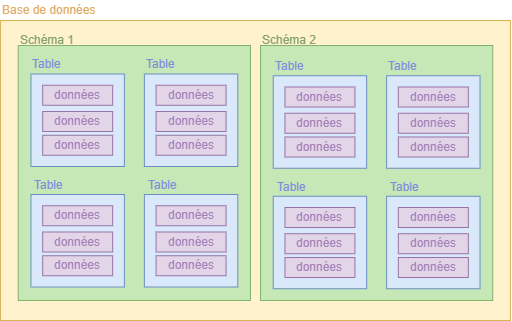
\includegraphics[width=\textwidth]{annexes/image1.png}

\section*{La base de données}

C'est la boîte englobante. L'instruction correspondante est~:

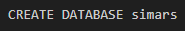
\includegraphics{annexes/image2.png}

Sa présence est optionnelle dans le script, ce qui veut dire que si elle
est absente, restaurer la base de données nécessitera de créer la boîte
englobante avant de lancer le script.

\section*{Les schémas}

Un schéma est un ensemble de tables. Un schéma sert à organiser les
tables dans la base de données par thématique ou à gérer des droits
d'accès différencié à une partie de la base seulement pour certaines
catégories d'utilisateurs (en ne lui donnant accès qu'à un seul schéma).
Des tables insérées dans des schémas différents peuvent donc être liées.

La présence de schéma(s) est optionnelle. Il existe un schéma par
défaut, \emph{public}, qui n'est pas déclaré s'il est le seul schéma.

L'instruction correspondante~est~:

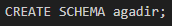
\includegraphics{annexes/image3.png}

Ici, le schéma s'appelle agadir.

Dans les exports à plat d'une base de données qui contenait des schémas,
il est possible que l'on trouve des dossiers correspondants aux schémas,
comme ici~:

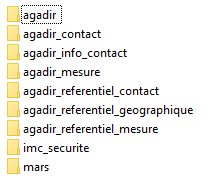
\includegraphics{annexes/image4.png}

Chacun des dossiers correspond à un schéma, et contient les tables
contenues dans le schéma.

\section*{Les tables}

Les tables contiennent les données de la base.

L'instruction correspondante~est :

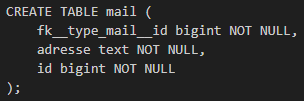
\includegraphics{annexes/image5.png}

Le nom de la table suit la déclaration CREATE TABLE. Ici, la table
s'appelle mail.

La déclaration de la colonne suit toujours le même ordre~: nom de la
colonne (obligatoire) -- nature de la données (obligatoire) --
contrainte (optionnel~; il peut y en avoir plusieurs). Pour la colonne
id, on a donc~:

fk\_type\_mail\_id bigint NOT NULL

c'est-à-dire~:

\begin{itemize}
	\item
	nom de colonne~: fk\_type\_mail\_id
	\item
	nature de la donnée~: grand entier
	\item
	contrainte~: la donnée doit être renseignée (la case ne peut pas être
	vide)
\end{itemize}

Les types de données les plus utilisées sont les suivants\footnote{Les autres types de données dans PostgreSQL 17 sont trouvables ici~: \href{https://docs.postgresql.fr/17/datatype.html}{Chapitre~8.~Types de données}}~:

\begin{table}[h]
	\centering
	\begin{tabular}{|l|l|}
		\hline
		\textbf{Noms des types de données} & \textbf{Signification} \\
		\hline
		smallint, integer, bigint & Nombre \\
		\hline
		Boolean & Valeur vrai/faux (\emph{true}/\emph{false}) \\
		\hline
		character varying(\emph{\textbf{n}}), varchar(\emph{\textbf{n}}) & Suite de caractères avec un nombre maximal de caractères \\
		\hline
		Text & Suite de caractères de longueur illimitée \\
		\hline
		Date & Date \\
		\hline
		Timestamp & Date et heure \\
		\hline
	\end{tabular}
	\caption{Types de données et leur signification}
\end{table}



Attention~: les données sont versées dans la table par une instruction
séparée.

\section*{Les données}

Instruction correspondante~:

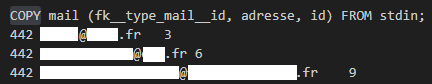
\includegraphics{annexes/image6.PNG}

Les données sont copiées de l'entrée (FROM stdin~; ici stdin est le
dump) à la table de destination, ici mail (indiqué après COPY, comme
dans \emph{copy in}\ldots{} en anglais). Les données sont copiées
suivant l'ordre de déclaration des colonnes~:

\begin{itemize}
	\item
	fk\_type\_mail\_id est indiqué la première, donc la première colonne
	de données (ici les 442) sera copiée à l'intérieur
	\item
	adresse est indiquée la deuxième, donc la deuxième colonne de données
	(les adresses mail) sera copiée à l'intérieur
	\item
	etc.
\end{itemize}

Chaque retour à la ligne représente un nouvel enregistrement. Les
valeurs NULL peuvent être représentées par un \textbackslash N ou NULL.

/!\textbackslash~: bien que moins répandu, un autre type d'instruction
existe pour copier les données~:

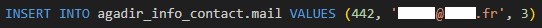
\includegraphics{annexes/image7.PNG}

«~Insère dans la table mail du schéma agadir\_info\_contact les valeurs
442, xxxxx@xxxx.fr, 3~».

Les données sont copiées suivant l'ordre de déclaration des colonnes.
Cette instruction est répétée pour toutes les lignes de toutes les
tables.

\section*{Les contraintes de clef étrangère (\emph{foreign key}/FK)}~

Ces contraintes, qui relient une clef primaire dans la table A à une
clef étrangère dans la table B, sont ce qui permet au programme de
relier les tables entre elles.

Instruction correspondante~:

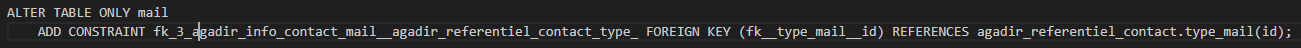
\includegraphics[width=\textwidth]{annexes/image8.png}

C'est avec cette instruction qu'on identifie à quelle table est reliée
la table mail. Elle est obligatoire quand il y a des liens de table à
table. Si une table contient plusieurs clefs étrangères, alors il y a
plusieurs déclarations de contrainte.

Lisons d'élément à élément~:

\begin{itemize}
	\item
	ALTER TABLE ONLY~mail~: on change quelque chose dans la table mail. Le
	ONLY est optionnel
	\item
	ADD CONSTRAINT~: on ajoute une contrainte
	\item
	fk\_3\_agadir (\ldots)~: le nom de la contrainte
	\item
	FOREIGN KEY~: on ajoute une relation de la table mail à une autre avec
	une clef étrangère
	\item
	(fk\_\_type\_mail\_\_id)~: le nom de la colonne qui contient la clef
	étrangère
	\item
	REFERENCES~: fait référence à
	\item
	agadir\_referentiel\_contact.type\_mail(id)~: la colonne id de la
	table type\_mail, qui fait partie du schéma
	agadir\_referentiel\_contact (si la base de données n'était pas
	organisée en schémas, on trouverait uniquement type\_mail(id))
\end{itemize}

La clef primaire à laquelle cette contrainte fait référence est déclarée
ici~:

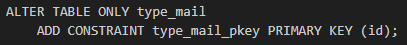
\includegraphics{annexes/image9.png}

Autrement «~Fait un changement dans la table type\_mail~;~»,
c'est-à-dire que le script ajoute une contrainte du nom de
«~type\_mail\_pkey~» pour transformer en clef primaire les
enregistrements de la colonne «~id.~»

Avec ces déclarations clef primaire/clef étrangère, on peut reconstituer
les liens entre les tables (ex. extrait du modèle de données généré avec
dbeaver)~:

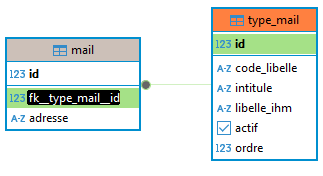
\includegraphics{annexes/image10.png}

Les id dans l'export csv de la table mail\_type~:

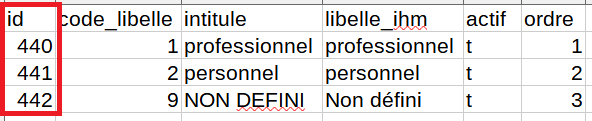
\includegraphics{annexes/image11.png}

Les id de la table mail\_type que l'on retrouve dans la table mail~:

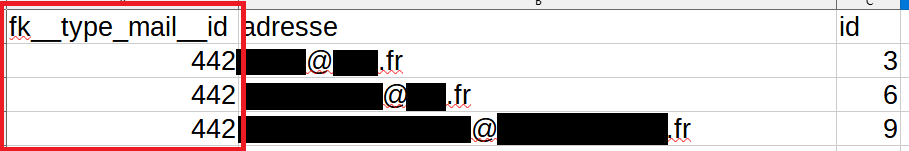
\includegraphics[width=\textwidth]{annexes/image12.png}

En reliant ces tables, on peut conclure qu'on ne sait pas si les
adresses mails visibles sur cette capture sont des adresses personnelles
ou professionnelles (elles ont la valeur 442, soit NON DEFINI dans la
table correspondante).
